\documentclass[12pt, a4paper]{article}

\setlength{\headheight}{15pt}

\usepackage{float}
\usepackage[table]{xcolor}

%%%%%%%%%%%%%%%%%%%%%%%%%%%%%%%%%%%%%%%%%
% House Style Structure
%%%%%%%%%%%%%%%%%%%%%%%%%%%%%%%%%%%%%%%%%

%----------------------------------------------------------------------------------------
% PACKAGES AND OTHER CONFIG
%----------------------------------------------------------------------------------------
\usepackage[english]{babel}
\usepackage{microtype}
\usepackage{amsmath,amsfonts,amsthm}
\usepackage{titling}

% TikZ
\usepackage{tikz}
\usetikzlibrary{positioning, calc, fit, arrows.meta}

\usepackage[svgnames]{xcolor}
\usepackage[hang, small, labelfont=bf, up, textfont=it]{caption}
\usepackage{array}
\usepackage{tabularx}
\usepackage{booktabs}
\usepackage{lastpage}
\usepackage{graphicx}
\usepackage{enumitem}
\setlist{noitemsep}

%----------------------------------------------------------------------------------------
% MARGINS AND SPACING
%----------------------------------------------------------------------------------------
\usepackage{geometry}
\geometry{
    top=1.0cm,
    bottom=1.0cm,
    left=1.5cm,
    right=1.5cm,
    includehead,
    includefoot,
}
\setlength{\columnsep}{7mm}

%----------------------------------------------------------------------------------------
% FONTS
%----------------------------------------------------------------------------------------
\usepackage[T1]{fontenc}
\usepackage[utf8]{inputenc}
\usepackage{XCharter}

%----------------------------------------------------------------------------------------
% HEADERS AND FOOTERS (house style)
%----------------------------------------------------------------------------------------
\usepackage{fancyhdr}
\pagestyle{fancy}
\renewcommand{\headrulewidth}{0.0pt}
\renewcommand{\footrulewidth}{0.4pt}

\renewcommand{\sectionmark}[1]{\markboth{#1}{}}

% Headers
\lhead{}
\chead{\textit{\thetitle}}
\rhead{}

% Footers
\lfoot{}
\cfoot{}
\rfoot{\footnotesize Page \thepage\ of \pageref{LastPage}}

\fancypagestyle{firstpage}{
    \fancyhf{}
    \renewcommand{\footrulewidth}{0pt}
}

%----------------------------------------------------------------------------------------
% ABSTRACT HELPERS
%----------------------------------------------------------------------------------------
\usepackage{lettrine}
\usepackage{fix-cm}
\usepackage{xstring}
\newcommand{\initial}[1]{\lettrine[lines=3,findent=4pt,nindent=0pt]{\color{Black}{#1}}{}}
\newcommand{\lettrineabstract}[1]{\StrLeft{#1}{1}[\firstletter]\initial{\firstletter}\textmd{\StrGobbleLeft{#1}{1}}}


\title{Data Science Execution Framework}
\newcommand{\theothertitle}{Data Science Infrastructure, Model Management, and Analytics Platform}
\author{Matt Pappas}
\date{September 11, 2025}

\begin{document}

%----------------------------------------------------------------------------------------
%\tEXECUTIVE ABSTRACT (HOUSE STYLE)
%----------------------------------------------------------------------------------------
\begin{center}

    \vspace{0.5em}

    {\LARGE \bfseries \MakeUppercase{Executive Abstract} \par}

    \vspace{0.25em}

    {\small Data Science Execution Framework Built on the Kiewit Intelligence Platform}

    \vspace{0.25em}

    {\small \emph{Kiewit Data Services}}

    \vspace{0.5em}
    
\end{center}

\begin{table}[h!]
\centering
\renewcommand{\arraystretch}{1.3}
\begin{tabularx}{\textwidth}{@{}
  >{\raggedright\arraybackslash\relax}p{2.8cm}
  X@{}}
\toprule
\textbf{Framework Requirement} & \textbf{Executive Summary} \\
\midrule

\textbf{Storage Abstraction (APIs)} &
\begin{itemize}[leftmargin=*, nosep]
  \item Enables enterprise-scale resilience by isolating systems through API contracts - when source systems change, only the API needs updating rather than hundreds of downstream consumers
  \item Centralizes security, governance, and versioning at the API layer
  \item Enables consistent schemas, documentation, and discoverability (API catalog)
  \item Enhances auditability and observability of data access patterns
\end{itemize} \\
\midrule

\textbf{Event-Driven (Source-Initiated)} &
\begin{itemize}[leftmargin=*, nosep]
  \item Source systems initiate end-to-end pipelines for lower latency and higher throughput
  \item Aligns with Caterpillar’s source-triggered data movements to increase velocity
  \item Reduces orchestration code complexity and improves reliability (idempotency/backpressure)
  \item Standardizes trigger $\rightarrow$ transform $\rightarrow$ serve patterns for apps and ML
  \item Strengthens end-to-end observability from event to product
  \item Pipeline visualizer: end-to-end DAGs improve learnings for data science; cited by Caterpillar Digital executives as a key enabler
\end{itemize} \\
\midrule

\textbf{Extensibility (Iceberg + Polaris)} &
\begin{itemize}[leftmargin=*, nosep]
  \item Iceberg tables on cloud object storage enable N‑way parallel reads for High Performance Compute (HPC) workloads
  \item Direct access to Silver (Iceberg) for data science and analytics; avoid Snowflake for sustained HPC cost/perf
  \item Polaris catalog provides open, engine‑agnostic governance and interoperability
  \item Gold is product‑modeled for business consumption and performance
  \item Partitioning/compaction and metadata‑based pruning sustain throughput at scale
  \item Cost posture and governance: favor object storage + Iceberg to control storage/egress costs; Polaris provides RBAC and centralized policies
\end{itemize} \\
\midrule

\textbf{Data Integrity \& Quality (Prism)} &
\begin{itemize}[leftmargin=*, nosep]
  \item On‑save validation: business logic applied at ingest so stored data is inference‑ready
  \item Regression fits detect subtle anomalies by identifying samples that deviate from expected trends and thresholds
  \item Closed‑loop “chain of evidence” for correction; auditable outcomes and decisions
\end{itemize} \\
\bottomrule
\end{tabularx}
\caption{Executive abstract: four foundational requirements for the Kiewit Intelligence Platform}
\label{tab:dsx_exec_overview}
\end{table}

\thispagestyle{empty}
\newpage

%----------------------------------------------------------------------------------------
%\tTITLE PAGE (HOUSE STYLE)
%----------------------------------------------------------------------------------------
\begin{center}
    \noindent\rule{\linewidth}{2pt} % Top rule

    \vspace{0.5em}

    {\LARGE \bfseries \MakeUppercase{\thetitle} \par}

    \vspace{0.25em}

    {\small \theothertitle}

    \vspace{0.5em}
    
    \noindent\rule{\linewidth}{2pt} % Bottom rule

    \vspace{0.5em}

    % Left-aligned author/date block
    \makebox[\linewidth][l]{%
      \begin{tabular}{@{} l @{}}
        \textbf{Author:} Matt Pappas \\ [6pt]
        \textbf{Date:} September 19, 2025 \\ [6pt]
        \textbf{Reviewers:} \\
        \hspace{1em}Austin Anderson, Sr. Data Scientist \\
        \hspace{1em}Jack Bruck, Sr. Data Scientist \\
        \hspace{1em}Gayatri Kallepalle, Manager KDS Data Engineering \\
        \hspace{1em}Eric Sornson, Manager KDS Web Services \\
        \hspace{1em}Dave Freeman, VP Data and Finance

      \end{tabular}%
    }

    \vspace{0.5em}

    \noindent\rule{\linewidth}{2pt} % Bottom rule
\end{center}

\setcounter{page}{1}
\thispagestyle{firstpage}

%----------------------------------------------------------------------------------------
% CONTENT (unchanged below)
%----------------------------------------------------------------------------------------

\section{Storage Abstraction: API-First Data Access}

\subsection{Executive Summary}
For several years, our data science team has successfully used APIs to decouple machine learning models from consuming applications. This proven pattern has enabled continuous model improvements without disrupting application development. Building on this success and Caterpillar's enterprise implementation, we can now scale these benefits organization-wide:

\begin{itemize}[leftmargin=*, nosep]
    \item Stable contracts: APIs abstract physical storage and schema drift behind versioned interfaces, proven through years of model upgrades
    \item Centralized monitoring: Azure Application Insights provides unified telemetry, tracing, and metrics for both data science models and applications
    \item Discoverability: FastAPI's built-in Swagger documentation provides interactive API exploration and standardizes onboarding
    \item Scalable Compute: Purpose-built APIs enable parallel processing and optimized compute resources for both ML training and application serving
    \item Observability: access patterns, errors, and latency are measurable at the API tier
\end{itemize}

\subsection{API Catalog (FastAPI Swagger / OpenAPI with Centralized Discovery)}
FastAPI's built-in Swagger UI (OpenAPI) provides immediate, auto-generated documentation per service. Beyond documentation, FastAPI offers high performance on par with NodeJS and Go, automatic data validation, editor support with autocompletion, and modern Python type hints. It is production-ready with automatic security via OAuth2 and JWT tokens. This meets near-term needs for discoverability and developer velocity. Our architecture centers on domain-specific application monorepos (scheduling, estimating, etc.) where front-end developers have direct access to Data Engineering API code within their domain. This eliminates API-to-API chaining by ensuring each API endpoint maps 1:1 with optimized Iceberg tables, delivering fast data access without middleware layers. Document workflows leverage NextJS components with direct data lake access where appropriate. To address enterprise-scale discoverability, we will build a centralized catalog that aggregates all FastAPI endpoints across domains, providing searchable metadata, usage patterns, and unified documentation. This approach allows us to maintain the development velocity of distributed FastAPI services while ensuring organization-wide visibility and governance. Our discussions with Caterpillar Digital revealed they successfully manage over 100,000 API routes through Apigee, demonstrating proven enterprise patterns we can adapt to our centralized catalog solution.

\begin{figure}[H]
    \centering
    \includegraphics[width=\textwidth]{01_swagger_docs.png}
    \caption{FastAPI Swagger (OpenAPI) catalog (deployed in Azure). Auto-generated docs with schemas, examples, and try-out capability accelerate adoption; architecture leaves the door open to Apigee as a central API catalog and gateway.}
    \label{fig:api_catalog}
\end{figure}

\subsection{Reference Data Flow}
The reference pattern is source-triggered and API-mediated, ensuring clear ownership at each hop and consistent contracts end-to-end.

\begin{figure}[H]
    \centering
    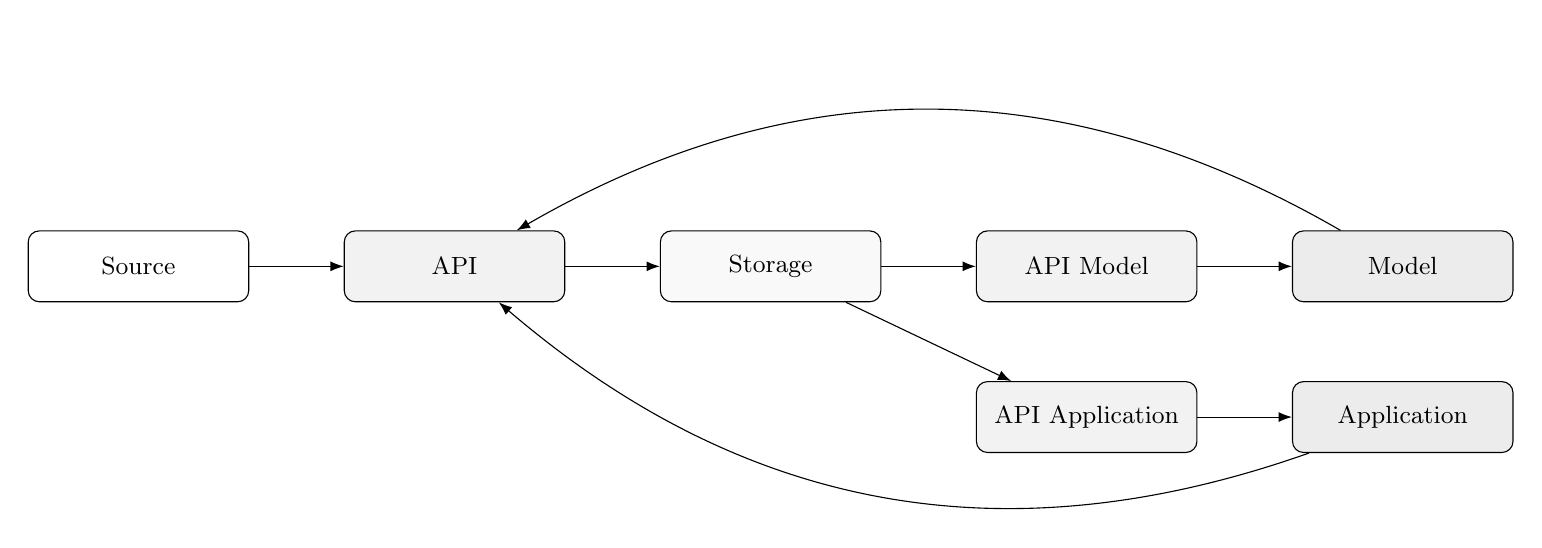
\begin{tikzpicture}[
        node distance=12mm,
        every node/.style={font=\small},
        box/.style={draw, rounded corners, align=center, inner sep=4pt, minimum width=28mm, minimum height=9mm},
        api/.style={box, fill=gray!10},
        store/.style={box, fill=gray!5},
        proc/.style={box, fill=gray!15}
    ]
        % Nodes
        \node[box] (source) {Source};
        \node[api, right=of source] (api) {API};
        \node[store, right=of api] (storage) {Storage};
        \node[api, right=of storage] (apimodel) {API Model};
        \node[api, below=10mm of apimodel] (apiapp) {API Application};
        \node[proc, right=of apimodel] (model) {Model};
        \node[proc, right=of apiapp] (app) {Application};

        % Arrows
        \draw[->, >=Latex] (source) -- (api);
        \draw[->, >=Latex] (api) -- (storage);
        \draw[->, >=Latex] (storage) -- (apimodel);
        \draw[->, >=Latex] (storage) -- (apiapp);
        \draw[->, >=Latex] (apimodel) -- (model);
        \draw[->, >=Latex] (apiapp) -- (app);
        
        % Return paths from Model and App back to Storage via API
        \draw[->, >=Latex] (model) to[bend right=30] (api);
        \draw[->, >=Latex] (app) to[bend left=30] (api);
    \end{tikzpicture}
    \caption{Reference pattern: Data flows from source through APIs and storage to models and applications, with feedback loops back through APIs}
    \label{fig:storage_flow}
\end{figure}

\begin{figure}[H]
    \centering
    \includegraphics[width=\textwidth]{landscape_level_2r1.png}
    \caption{Platform landscape (level 2): end-to-end view across sources, API ingress, Bronze/Silver/Gold storage, Polaris governance, and serving for applications and ML.}
    \label{fig:landscape_level2}
\end{figure}

\section{Event-Driven: Source-Initiated Data Movements}

\subsection{Executive Overview}
An event-driven architecture increases pipeline velocity and reliability by moving initiation to the source system. This pattern reduces orchestration complexity, shortens end-to-end latency, and improves observability from trigger to product. Consistent with Caterpillar’s approach, source-triggered movements standardize the flow from ingest to serve for both applications and machine learning.

\subsection{Source-Initiated Pipeline Pattern (Caterpillar-Inspired)}
The source system initiates the end-to-end pipeline (e.g., HTTP POST to ingest API), which validates, persists, and then triggers downstream transformations and serving. This aligns with Caterpillar's source-triggered movement model that increased data velocity while simplifying operational ownership across domains. Rather than layering SQL views that obscure business logic through nested abstractions, KDS data scientists advocate for consolidated, version-controlled transformation scripts that make all business rules explicit and traceable. Each pipeline becomes a single, well-documented artifact where transformations are centralized, commented, and free of hard-coded values—eliminating the archaeological work of tracing logic through multiple database layers. A built-in pipeline visualizer exposes these transparent end-to-end DAGs to accelerate data science learning and incident triage—cited by Caterpillar Digital executives as a key enabler.

\begin{figure}[H]
    \centering
    \includegraphics[width=\textwidth]{01_flow.png}
    \caption{Source-initiated orchestration: events flow from source to API ingest, storage, transformation, and serving with clear ownership and standardized contracts.}
    \label{fig:source_initiated_flow}
\end{figure}

\subsection{Velocity and Code Complexity}
\begin{figure}[H]
    \centering
    \includegraphics[width=\textwidth]{raptor_engines.png}
    \caption{SpaceX Raptor engine's increasingly complex wiring reflects our data architecture's evolution - adding new connections and pathways to handle growing capabilities rather than fundamentally redesigning the system}
    \label{fig:raptor_analogy}
\end{figure}

Just as SpaceX's Raptor engine evolved from a maze of individual wires to streamlined pathways, our data architecture must undergo similar simplification. Over 15 years, we've layered on complexity - from on-premise SQL Server to Teradata to Snowflake to Data Lake - each transition adding new connections rather than streamlining existing ones. Like the Raptor's refined design, we need to consolidate these scattered pathways into robust, simplified flows. By eliminating redundant connections and standardizing data access through consistent API routes, we can achieve greater velocity with less complexity. This means replacing brittle point-to-point integrations with resilient, well-defined FastAPI interfaces that provide standardized routes for accessing the data lake. Rather than building a single monolithic API, we establish consistent patterns for authentication, authorization, and workload management across distributed FastAPI services that each handle specific data domains or functional areas.

\subsection{Orchestration and High-Performance Compute}
Our hybrid compute infrastructure combines on-premises GPU/CPU clusters with cloud resources to optimize both development and production workloads. Key benefits include:

Development teams get fast, local access to compute through dedicated on-premises hardware, similar to how construction crews need immediate access to equipment on-site. When local resources are fully utilized, workloads automatically burst to the cloud - like bringing in additional equipment from other sites during peak demand.

The orchestration layer (using tools like Dagster with Ray) acts as the central dispatch office, directing compute jobs to the right environment based on:
\begin{itemize}
    \item Available resources and capacity
    \item Where the data is located 
    \item Required response times
    \item Cost considerations
\end{itemize}

For specialized production needs, we maintain dedicated on-premises hardware with cloud elasticity - when local resources reach capacity, workloads automatically shift to cloud infrastructure. This hybrid approach ensures consistent performance by leveraging on-premises systems for standard workloads while seamlessly expanding to cloud resources during peak demand periods. Like a construction site that maintains core heavy equipment but can quickly source additional machinery when projects scale up, our infrastructure flexes to match computational needs without disrupting operations.

\subsection{ML Endpoints, Serving Pattern and Model Versioning}
Production ML serving is primarily delivered through Azure API endpoints, providing standardized access to features and model inference. This cloud-first approach leverages Azure's managed services for optimal scalability, monitoring, and cost efficiency. The serving infrastructure utilizes Azure Kubernetes Service (AKS) with GPU-enabled nodes for production workloads, enabling automatic scaling based on demand.

For development and experimentation purposes, data scientists can utilize on-premises Kubernetes clusters to develop, fine-tune and test models before promoting them to production Azure endpoints. This development environment mirrors production configurations while providing faster iteration cycles.

Model versioning and reproducibility are ensured through:

\begin{itemize}
    \item Version control of model code, hyperparameters, and training scripts in Git
    \item Immutable storage of trained model artifacts in Azure Blob with versioned references
    \item Automated logging of training metrics, data lineage, and model performance
    \item Documentation generation capturing model architecture and training process
    \item Inference request/response logging with model version tracking
    \item Regular model snapshots stored with corresponding training data
\end{itemize}

This comprehensive versioning enables reconstruction of any model version, including:
\begin{itemize}
    \item The exact training dataset and feature engineering pipeline
    \item Model architecture, weights and hyperparameters
    \item Training environment configuration and dependencies
    \item Model evaluation metrics and validation results
    \item Deployment configuration and serving endpoints
\end{itemize}

Production workloads may utilize on-premises infrastructure by exception only, when justified by:
\begin{itemize}
    \item Strict data residency or regulatory requirements
    \item Ultra-low latency needs that cannot be met by cloud endpoints
    \item Specialized hardware dependencies not available in Azure
    \item Critical business continuity requirements
\end{itemize}

This pattern enables consistent consumption by applications and batch/real-time ML with unified governance, documentation, and observability guarantees across environments through Azure Arc integration. The versioning system ensures full reproducibility and auditability of model development through production deployment.

\begin{figure}[H]
    \centering
    \includegraphics[width=\textwidth]{01_flow_ml_endpoint.png}
    \caption{ML serving endpoints: standardized APIs power online inference and feature access with versioned contracts, model artifacts, and integrated monitoring across hybrid infrastructure.}
    \label{fig:ml_endpoints}
\end{figure}

\section{Extensibility: Iceberg Tables and Polaris Catalog}

\subsection{Executive Overview}
Extensibility is achieved by separating write-optimized ingest (Bronze) from read/serve-optimized tables (Silver/Gold) using Apache Iceberg and an open catalog (Polaris). This design enables schema evolution, time travel, ACID guarantees, and seamless interoperability with Snowflake (KDP) and other engines—while preserving performance and governance.

\subsection{Layered Storage Design}
\begin{itemize}[leftmargin=*, nosep]
    \item \textbf{Bronze (Write-Optimized Ingest)}: Blob containers and Data Lake paths optimized for high-throughput writes from sources; minimal transformation for durability and replay.
    \item \textbf{Silver (Iceberg Tables)}: Apache Iceberg provides table evolution, partitioning, time travel, and ACID—serving both applications and ML via stable iceberg tables.
    \item \textbf{Gold (Modeled for Products)}: Business-modeled tables optimized for analytics performance, curated with data architecture standards and cataloged for discoverability.
    \item \textbf{Open Catalog (Polaris)}: Central governance and open interoperability across engines (including Snowflake) using standardized table metadata.
    \item \textbf{Enterprise Interop (Snowflake / KDP)}: Iceberg tables integrate with broader enterprise datasets to enable cross-domain analytics without duplication.
    \item \textbf{Cost Posture}: Favor object storage + Iceberg for HPC reads and data science workloads to avoid sustained database storage and egress costs; reserve premium databases for productized Gold use cases.
\end{itemize}

\subsection{Cost Analysis: Database vs Iceberg Storage}
A key consideration in our storage strategy is cost optimization. Current database storage costs consume over 45\% of service expenses. While Iceberg tables have slower performance in high-update environments, our data science workloads predominantly involve temporal full loads—an ideal use case for Iceberg's architecture. 

\begin{figure}[H]
    \centering
    \includegraphics[width=\textwidth]{01_storage_cost.png}
    \caption{Cost comparison between traditional Azure SQL Database service (left) and Iceberg tables (right) for container API implementations, demonstrating significant storage cost savings with Iceberg.}
    \label{fig:storage_costs}
\end{figure}

\subsection{Bronze: Multi-Format Write-Optimized Storage}
\begin{figure}[H]
    \centering
    \includegraphics[width=\textwidth]{01_storage_silver.png}
    \caption{Bronze layer employs a hybrid storage approach, utilizing both Parquet and Iceberg formats based on workload requirements. While Parquet provides efficient memory-to-disk writes for standard API ingestion through hierarchical paths (e.g., blob containers $\rightarrow$ datalake $\rightarrow$ bronze $\rightarrow$ p6 $\rightarrow$ spread\_service $\rightarrow$ p6central $\rightarrow$ schedule\_id=22785/year=2025/month=09/day=04), select high-value datasets leverage Iceberg tables directly in Bronze for enhanced versioning and ACID guarantees during initial ingestion. This dual approach optimizes for both performance and data integrity based on business criticality.}
    \label{fig:bronze_paths}
\end{figure}

\subsection{Silver: Apache Iceberg for API-First Data Serving}
\begin{figure}[H]
    \centering
    \includegraphics[width=\textwidth]{01_storage_silver.png}
    \caption{Silver layer (Iceberg) serves as the primary data access tier through dual API endpoints: one optimized for data science model training/inference, and another for application consumption. This API-first design, backed by Iceberg's metadata management, enables consistent data access while maintaining time travel, schema evolution, and ACID guarantees. While these Silver objects can be promoted to Gold tier, their primary purpose is direct serving of data science and application workloads.}
    \label{fig:silver_iceberg}
\end{figure}

\subsection{Gold: Product-Modeled Data}
Gold is curated by data architecture to meet product management specifications. These certified datasets are tuned for analytics performance and cataloged for enterprise consumption.

\subsection{Polaris Catalog (Open Table Governance)}
\begin{figure}[H]
    \centering
    \includegraphics[width=\textwidth]{01_storage_polaris.png}
    \caption{Polaris catalog: open, engine-agnostic governance of Iceberg tables, enabling consistent discovery, role-based access control (RBAC), access policies, and lifecycle management.}
    \label{fig:polaris_catalog}
\end{figure}

\subsection{Snowflake (Kiewit Data Platform / KDP) Interoperability}
\begin{figure}[H]
    \centering
    \includegraphics[width=\textwidth]{01_storage_snowflake.png}
    \caption{Snowflake (KDP) interoperability: Iceberg tables interoperate with enterprise datasets for cross-domain analytics and downstream productization without duplication.}
    \label{fig:snowflake_kdp}
\end{figure}

\subsection{High-Performance Parallel Reads (Critical Cost Driver)}
Large-scale model training and inference jobs represent a significant operational cost, potentially reaching millions of dollars annually in cloud compute expenses. These workloads require massive parallel processing where hundreds or thousands of workers simultaneously access training data. The storage layer must efficiently handle this N-way parallel read pattern without becoming a bottleneck or cost center. While competitors like Caterpillar use expensive NoSQL solutions (DynamoDB), our cost-optimized approach leverages Apache Iceberg tables on cloud object storage. This architecture delivers the required performance through rich metadata management (manifests, partition specs), efficient columnar formats (Parquet), and intelligent data pruning—enabling distributed compute engines (Spark/Trino/Dask or native readers) to process data in parallel while avoiding unnecessary storage and compute costs.

To guarantee cloud-scale performance, we will:
\begin{itemize}[leftmargin=*, nosep]
    \item Design table layouts for parallelism: appropriate partitioning/bucketing and regular small-file compaction
    \item Enable predicate/column pruning and data skipping via Iceberg metadata and statistics
    \item Co-locate compute with object storage and use read caches where available
\end{itemize}
This requirement is non-negotiable: HPC workloads will overwhelm any storage tier that cannot scale out parallel reads; Iceberg on cloud object storage gives us that elasticity without introducing a separate NoSQL dependency.

\paragraph{Cost and Access Model}
For sustained HPC training/inference, routing Silver through Snowflake would be cost‑prohibitive and adds an extra hop. Our servers read Iceberg tables directly (e.g., Spark/Trino/Dask or native Iceberg readers) and expose results through APIs as needed. Data science accesses Silver directly via Iceberg—without Snowflake in the path—so parallel readers can fully utilize cloud object storage bandwidth at predictable cost.

\section{Data Integrity and Quality: Prism}

\subsection{Executive Overview}
Our lakehouse architecture unifies data storage and access through a consistent API layer, enabling both traditional business logic validation and advanced machine learning quality checks. Within this architecture, Prism serves as our specialized data quality subsystem, applying regression-based validation and maintaining closed-loop evidence chains. By abstracting the underlying Apache Iceberg storage through APIs, we ensure that all data—whether accessed for quality validation, analytics, or model training—adheres to consistent quality standards while maintaining the flexibility to evolve our storage strategy. This API-first approach allows us to encode complex business rules and leverage ML-driven quality checks without tightly coupling applications to specific storage implementations. Prism enforces on-save validation for all data intended for machine learning inference, applying business rules synchronously at ingestion so stored data is trusted and inference-ready.

\subsection{Core Principles}
\begin{itemize}[leftmargin=*, nosep]
    \item \textbf{API-First Integration}: Unified API layer enables consistent access across subsystems while avoiding Snowflake limitations and costs
    \item \textbf{Vendor Independence}: Apache Iceberg tables can be virtualized across cloud providers, preventing lock-in that would cost millions in application rewrites
    \item \textbf{Full ML Lifecycle}: Direct support for container serving, model hosting, and foundational AI models—capabilities Snowflake cannot provide
    \item \textbf{Cost-Optimized Storage}: Bronze layer data stored in cloud-native formats, avoiding expensive Snowflake storage fees for raw application data
\end{itemize}

\subsection{Regression-Based Quality Validation: The First Step in Closed-Loop Validation}
Quality issues often appear innocuous until plotted against correlated variables. Prism's regression-based validation serves as the critical first phase of our closed-loop quality system, automatically detecting issues that feed into our correction workflow:
\begin{itemize}[leftmargin=*, nosep]
    \item Correlation-aware rules identify data points that violate learned relationships (e.g., equipment costs vs. project size, labor rates vs. regional benchmarks).
    \item Contextual thresholds (by asset, site, environment) reduce false positives and route issues to appropriate teams.
    \item Violations automatically initiate the closed-loop correction process with reproducible evidence.
\end{itemize}

\subsection{Closed-Loop Chain of Evidence}
Building directly on regression-based validation findings, our closed-loop system ensures every detected issue reaches resolution. This replaces the common "hung loop" anti-pattern where estimators informally flag data errors in Atlas and fixes diverge across teams. Prism enforces a structured workflow within the Atlas estimating system:
\begin{itemize}[leftmargin=*, nosep]
    \item \textbf{Triage}: Automatically classify regression-detected errors in Atlas estimate records (e.g., invalid labor rates, missing equipment costs).
    \item \textbf{Correct}: Apply automated fixes to standardize rates or route to estimating team with validation context.
    \item \textbf{Verify}: Re-run regression validation on corrected records and attach evidence (cost deltas, rate comparisons).
    \item \textbf{Record}: Document the original regression finding, correction applied, approving estimator, and verification data in Atlas Prism.
\end{itemize}

\subsection{Governance, Lineage, and Data Architecture}
Our data architecture follows a tiered approach where Silver represents normalized and standardized data, Gold contains business-focused datasets, and Platinum represents certified data meeting the highest quality standards. Data lineage is comprehensively tracked through two key artifacts stored in our Alation data catalog:

\begin{itemize}[leftmargin=*, nosep]
    \item Directed Acyclic Graphs (DAGs) visualizing complete data flow from source systems through Bronze ingestion, Silver standardization, and Gold/Platinum business layers
    \item Detailed source-to-target mappings documenting transformations and business rules at each tier
    \item Quality SLOs (freshness, completeness, accuracy) monitored across tiers with elevated standards for Platinum certification
    \item Versioned APIs governing all data access to maintain consistency and auditability
\end{itemize}

\end{document}
